\documentclass[12pt, letterpaper]{report}
\usepackage{graphicx}
\usepackage{hyperref}
\usepackage{amssymb}
\usepackage{amsmath}
\usepackage{float}
\usepackage{mathtools}
\usepackage{enumitem}
\usepackage[margin=1in]{geometry}
\usepackage[figurename=Figura]{caption}
\usepackage[tablename=Tabla]{caption}
\usepackage{indentfirst}
\usepackage{biblatex}
\addbibresource{bibliografia.bib}

\title{Redes Bayesianas Gaussianas: Un estudio de la influencia de los contaminantes del aire en la salud de la población mexicana}
\author{ Romina Nájera Fuentes - A01424411 \\ Humberto Mondragón García - A01711912 \\ Juan Braulio Olivares Rodríguez - A01706880 \\ Edgar Andrey Balvaneda - A01644770
 \\ \\ Análisis de métodos de razonamiento e incertidumbre}
\date{7 de Septiembre del 2025}


\begin{document}
\maketitle
\section*{Abstract}
\newpage

\section*{Introducción}

La contaminación ambiental se ha convertido en una problemática crítica para la salud pública a nivel mundial. Según la Organización Mundial de la Salud, 9 de cada 10 personas respiran aire con altos niveles de contaminantes, y 4.2 millones de personas mueren al año a causa de la contaminación del aire del exterior. \cite{who2018}
\\

En México, en las zonas metropolitanas, como la Ciudad de México, Monterrey y Guadalajara, se reportan concentraciones elevadas de contaminantes provenientes del intenso tráfico vehicular, sus altas densidades poblacionales y la actividad industrial con pocas o nulas restricciones en la liberación de contaminantes en el ambiente. Si bien esta mezcla de contaminantes es compleja, ciertos de ellos son especialmente preocupantes por su impacto en la salud pública. Los datos de la SEMARNAT nos proveen de los siguientes contaminantes:
\\

El material particulado ($PM_{10}$ y $PM_{2.5}$) constituye uno de los contaminantes atmosféricos más nocivos para la salud. Proviene principalmente de procesos de combustión como los de vehículos o actividades industriales, es culpable de agravamiento de los síntomas del asma, deterioro de la función pulmonar y aumento del riesgo de cáncer de pulmón, garganta o laringe.\cite{airly}
\\

El dióxido de azufre ($SO_2$) es un gas que se produce principalmente por la quema de combustibles fósiles como el carbón y el petróleo. Su inhalación provoca irritación de las vías respiratorias y desencadena reacciones inflamatorias locales y sistémicas. \cite{ivhhn2003}
\\

El monóxido de carbono ($CO$), por su parte, es un gas inodoro y altamente tóxico que se produce principalmente por la combustión incompleta de gasolina, madera, carbón o gas. Su mecanismo de toxicidad se debe a su alta afinidad con la hemoglobina, lo que desplaza al oxígeno y disminuye la capacidad de transporte de este en la sangre. \cite{mayoclinic2025}
\\

Los óxidos de nitrógeno ($NOx$), que incluyen principalmente el dióxido de nitrógeno ($NO_2$) y el óxido nítrico ($NO$), se generan a partir de procesos de combustión como en vehículos motorizados, plantas eléctricas e industrias. Estos gases son potentes irritantes de las vías respiratorias, provocan inflamación bronquial y reducen la función pulmonar. \cite{atsdr2016}
\\

Por último, los compuestos orgánicos volátiles ($COV$) y el amoníaco ($NH_3$), aunque menos estudiados en comparación con los contaminantes anteriores, también tienen efectos relevantes en la calidad del aire y la salud. Se han vinculado con irritación ocular y respiratoria, así como con procesos de estrés oxidativo. \cite{atsdr2026} Los $COV$ provienen de solventes, combustibles, pinturas y procesos industriales, contribuyen junto con los $NOx$ a la formación de ozono troposférico. \cite{epa2025}
\\

Por la ya mencionada complejidad de los contaminantes, resulta necesario estudiar no solo su presencia ambiental, sino también sus repercusiones biológicas medibles en la población.
\\

El presente trabajo tiene como objetivo principal implementar un modelo probabilístico que permita identificar en qué medida estos contaminantes influyen en la salud de la población mexicana, analizando sus biomarcadores. Comprender la magnitud de este impacto, el origen de los contaminantes, y los componentes biológicos afectados es fundamental para el diseño de políticas públicas efectivas y estrategias de prevención.
\\

Para ello utilizamos los datos de muestras biológicas de la Encuesta Nacional de Salud y Nutrición (ENSANUT) 2022, y registros de contaminantes atmosféricos provenientes de la SEMARNAT.
\\

Existen diversos enfoques estocásticos que podemos utilizar para modelar la influencia de los contaminantes en los biomarcadores. Entre ellos se encuentran métodos como la regresión, que permite evaluar asociaciones entre variables, los procesos de Poisson, que modelan conteos de eventos discretos, y las simulaciones Monte Carlo, que permiten explorar el comportamiento de modelos complejos. Sin embargo, estas aproximaciones frecuentemente se centran en relaciones simples entre variables o en estructuras lineales, lo que limita su capacidad de capturar la red de dependencias entre las variables de este estudio. Frente a ello, las redes bayesianas gaussianas ofrecen una alternativa más flexible representando las relaciones de dependencia en forma de un grafo acíclico dirigido y modelar la incertidumbre mediante distribuciones gaussianas.

\section*{Metodología}

Una red bayesiana es definida como un grafo acíclico dirigido, conocido como DAG, $D=(V,E)$, en donde $V=\{X_1,X_2,...,X_n\}$ representa a las variables del problema, y E representa las relaciones de dependencia entre las variables. Asimismo, se cuenta con P, el conjunto de distribuciones de probabilidad asociadas a cada nodo.
\\

Se utilizará una red bayesiana de tipo gaussiana, la cual es utilizada para modelar variables aleatorias continuas que siguen una distribución normal. En este caso, la distribución conjunta de las variables del problema es normal multivariada; es decir, sigue una distribución $N(\mu, \Sigma)$, siendo $\mu$ el vector de medias y $\Sigma$ la matriz de covarianzas. \cite{tesis}
\\

En la versión gaussiana de la red bayesiana, los nodos raíz, o nodos sin padres, siguen marginalmente una distribución univariada normal. Los demás nodos siguen de manera marginal una distribución condicionada normal, con una media que se representa a través de un modelo lineal respecto a las medias de los padres, y con una varianza propia \cite{scutari2021bayesian}.
\\

Entre las variables presentadas en la ENSANUT, se encuentra información sociodemográfica de las personas encuestadas, como el sexo, la edad, la zona de residencia, el acceso a servicios de salud pública, entre otros. Sin embargo, de estos solamente se tomará en cuenta la edad, que es una variable que se puede considerar continua, y el lugar en el que se reside, para asignar los niveles de contaminantes a los que los encuestados se exponen de manera constante.
\\

Además de la información sociodemográfica, la encuesta también contiene información relacionada con biomarcadores. Estos incluyen los niveles de ácido úrico, albúmina, colesterol HDL y LDL, colesterol total, creatinina, glucosa, insulina, proteína C reactiva, triglicéridos, hemoglobina glucosilada, ferritina, folato, homocisteina, receptor de transferrina, vitamina B12 y vitamina D de los encuestados. Si bien se cuenta con más información, estas variables son las que son continuas, condición necesaria en las redes bayesianas gaussianas, por lo que el impacto en la salud se determinará solamente con estas variables.
\\

Con la información de la SEMARNAT, como se mencionó previamente en la introducción, se utilizarán los niveles de los contaminantes $SO_2$, $CO$, $COV$, $NOx$, $PM_{10}$ y $PM_{2.5}$ medidos en los municipios de cada estado del país. Los contaminantes se dividen en diferentes tipos de fuentes causantes, que son las fuentes fijas, de área, móviles carreteros, móviles que no circulan por carretera y naturales. Por observación del Dr. Ernesto Reyes Villegas, experto en calidad del aire, estas fuentes son complementarias, por lo que la suma de los contaminantes en cada fuente es equivalente a la contaminación total en dicho municipio. Sin embargo, en vista de que no todos los municipios presentan información completa en las fuentes fijas y las fuentes naturales, se considerará que el nivel de contaminación a la que se somete una persona que reside en un municipio, es igual a la suma de la contaminación de fuentes de área, de móviles carreteros y de móviles que no circulan por carretera para cada contaminante por municipio.
\\

Las variables seleccionadas son exclusivamente continuas, con el propósito de utilizar la red bayesiana gaussiana. Agregar una variable categórica, como lo podría ser el sexo de la persona encuestada, representaría utilizar un modelo distinto al aquí presentado. Una manera de realizarlo es a través de la discretización de las variables continuas. Sin embargo, para una mayor precisión, la discretización se tendría que llevar con múltiples categorías para cada variable, lo cual incrementa la complejidad del modelo y su tiempo de cómputo. \cite{cowell}
\\

Otra manera de realizar el modelo con la combinación de variables discretas y continuas es a través de una red bayesiana mixta. En esta, los nodos discretos siguen una distribución multinomial, y sus nodos padres pueden ser solamente otras variables discretas. En cambio, los nodos continuos simplemente siguen una distribución normal, cuando ninguno de sus nodos padre son discretos; y siguen un conjunto de distribuciones normales, cada una para cada posible combinación de las variables de las que dependen, en caso de tener alguna variable discreta como nodos padre. \cite{scutari2021bayesian}
\\

Utilizando estas variables, se consultará a especialistas en las áreas de medicina y de bioquímica, quienes apoyarán en la realización de la red bayesiana gaussiana, seleccionando las variables de interés, y proponiendo las relaciones que consideren relevantes.
\\

Con ello, se generarán 3 DAGs, las cuales serán ajustadas a los datos para ser posteriormente comparadas entre sí a través del Criterio de Información Bayesiano (BIC), el cual considera la verosimilitud y la complejidad de cada modelo para asignar un puntaje que se busca maximizar  \cite{scutari2021bayesian}, y del Criterio de Información Akaike (AIC), el cual considera los mismos parámetros que el BIC, pero penaliza en menor escala a la complejidad del modelo.
\\

Estos criterios de información se calculan de la siguiente manera:
\\
\begin{equation}
AIC = -2 \ln(\hat{L}) + 2k
\label{eq:aic}
\end{equation}

\begin{equation}
BIC = -2 \ln(\hat{L}) + k \ln(n)
\label{eq:bic}
\end{equation}
\\
Después de seleccionar un modelo óptimo en base al puntaje BIC, se formarán 3 preguntas a resolver con dicha red bayesiana, las cuales se propondrán con el apoyo de los especialistas contactados para la propuesta de las redes.

\section*{Aplicación}

La primera propuesta de la DAG fue dada por la estudiante de medicina Leslie Aleydis Ocampo Hernández, quien recalcó el efecto de los contaminantes en el aumento de la proteína C reactiva ($pcr$), debido a la inflamación que estos generan. Asimismo, estableció el efecto que tiene el material particulado ($PM_{10}$ y $PM_{2.5}$) y el amoníaco ($NH_3$) en los niveles de ácido úrico y creatinina, debido al efecto en los riñones dada por la inflamación generada por estos contaminantes. En la Figura \ref{fig:dag1} se puede observar el grafo generado con la guía de la Dra. Ocampo.

\begin{figure}[H]
    \centering
    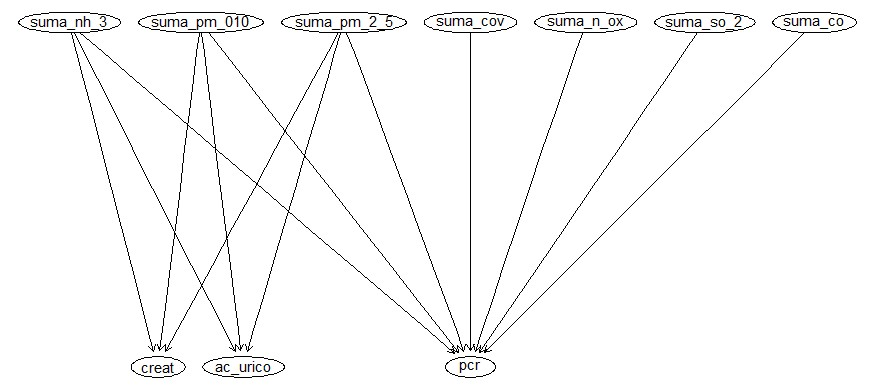
\includegraphics[width=\linewidth]{imgs/dag1.jpg}
    \caption{Grafo propuesto con el apoyo de la Dra. Ocampo.}
    \label{fig:dag1}
\end{figure}

La segunda propuesta para el grafo se obtuvo con ayuda de la Dra. Ma. Silvia Rodríguez López y del Dr. Ricardo Cano Pérez, quienes no consideraron que hubiera relación relevante entre el monóxido de carbono ($CO$) y los compuestos orgánicos volátiles ($COV$), respecto a alguno de los biomarcadores. Los demás contaminantes consideraron que todos influyen en la proteína C reactiva, en la ferritina y en el ácido úrico. Asimismo, decidieron añadir la edad como un factor que también influye a los niveles de los 3 biomarcadores mencionados. En la Figura \ref{fig:dag2} se observa el grafo generado con las observaciones realizadas por ambos doctores.

\begin{figure}[H]
    \centering
    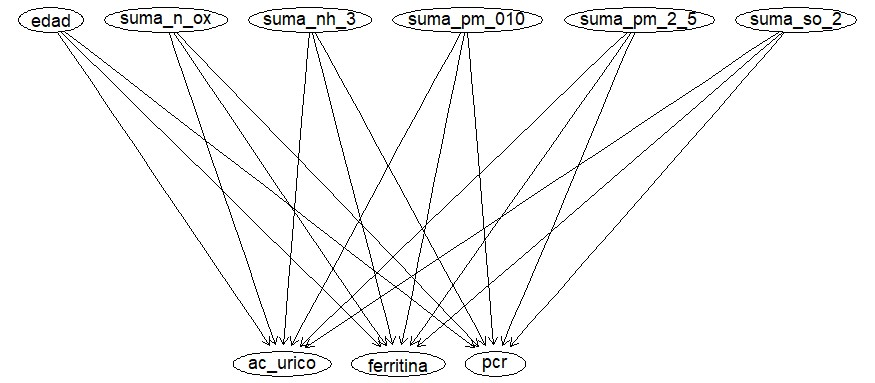
\includegraphics[width=\linewidth]{imgs/dag2.jpg}
    \caption{Grafo propuesto con el apoyo de la Dra. Rodríguez y el Dr. Cano.}
    \label{fig:dag2}
\end{figure}

La tercer propuesta de DAG se obtuvo con la ayuda del estudiante de medicina Jean Emmanuel Zabre Pando, quien estableció el efecto de los contaminantes como posible generador de inflamación, aumentando el nivel de proteína C reactiva, y el impacto del aumento de esta proteína, así como de los niveles de material particulado, en el metabolismo, particularmente en los triglicéridos. Posterior a ello, estableció las relaciones entre múltiples biomarcadores, información con la cual se generó la DAG de la Figura \ref{fig:dag3}.

\begin{figure}[H]
    \centering
    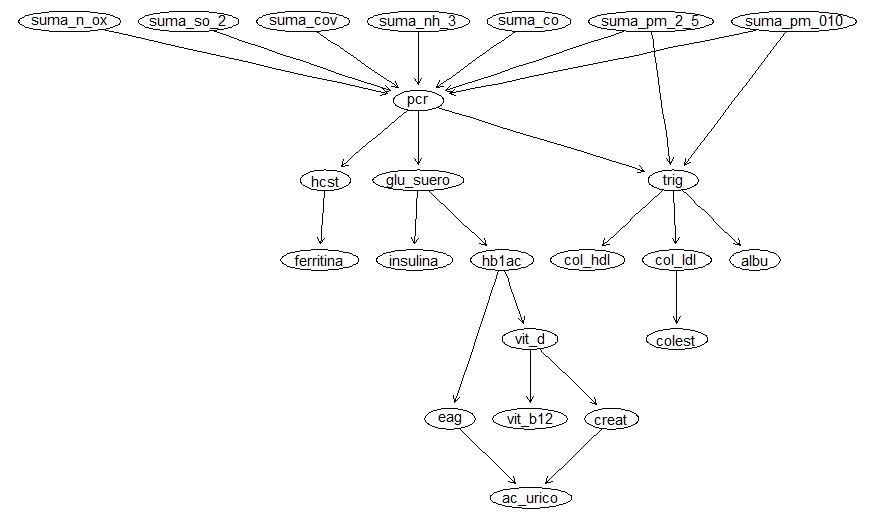
\includegraphics[width=\linewidth]{imgs/dag3.jpg}
    \caption{Grafo propuesto con el apoyo del Dr. Zabre.}
    \label{fig:dag3}
\end{figure}

Evaluando los modelos en los criterios de información seleccionados, se obtuvieron los resultados de la Tabla \ref{tab:scores}. Como ambos criterios se buscan maximizar para determinar un mejor modelo, los resultados muestran ser consistentes entre ambos criterios. Es decir, se puede concluir que el segundo modelo resultó en los valores más altos de los criterios, por lo que es la DAG con mejor ajuste entre las propuestas. Por otro lado, el tercer modelo tuvo los resultados más bajos, lo cual quiere decir que fue el que tuvo un peor ajuste a los datos. Esto se puede deber a la diferencia en complejidad de los modelos, puesto que el segundo modelo es el que tiene una menor cantidad de nodos, mientras que el tercer modelo es el que utiliza una mayor cantidad de variables. Sin embargo, los puntajes de los criterios también se ven influenciados por la verosimilitud del modelo, por lo que un menor puntaje también podría indicar un mal ajuste.

\begin{table}[H]
    \centering
    \begin{tabular}{|c|c|c|}
        \hline
        Modelo & BIC & AIC \\
        \hline
        1 & $-42502.98$ & $-42418.14$ \\
        \hline
        2 & $-32122.3$ & $-32027.29$ \\
        \hline
        3 & $-77035.66$ & $-76779.56$ \\
        \hline
    \end{tabular}
    \caption{Criterios de información bayesiano y akaike en los modelos propuestos.}
    \label{tab:scores}
\end{table}


En una red bayesiana gaussiana lineal, como la aquí utilizada, se asume que la media de la distribución normal es una combinación lineal de sus nodos padre; en un modelo no paramétrico, no se impone la regresión lineal para la media, sino que se usan splines o procesos más flexibles que se adaptan a los datos. Como el modelo tiene más “libertad” en los modelos no paramétricos para captar las irregularidades de los datos, la verosimilitud suele aumentar.\\

En un modelo paramétrico $k$ es bajo, (coeficientes + varianzas), pero en un modelo no paramétrico, $k$ tiende a ser más alto. Por ejemplo, en splines, aumentan la cantidad de parámetros\\

Como lo mencionamos anteriormente, en un modelo no paramétrico la verosimilitud suele aumentar, y como la penalización por los parámetros, que podemos observar en la fórmula de AIC\ref{eq:aic} se comporta como $2k$, normalmente la mejora en la verosimilitud lo compensa, por lo que AIC suele ser más bajo. (mejor)\\

En BIC, la verosimilitud también mejora, pero la penalización cambia \ref{eq:bic} , si $n$ es pequeño (número de datos), $ln(n)$ no es tan grande y la penalización puede matar al modelo no paramétrico, en cambio, si $n$ es grande, la verosimilitud aumentada puede compensar la penalización. Por lo que dependiendo de $n$ puede mejorar o no.\\

Como podemos darnos cuenta, el modelo que dio un mejor resultado para las métricas planteadas fue el propuesto en colaboración con la Dra. Silvia, por lo tanto, a partir de las variables relacionadas en esta DAG podemos plantear ciertas preguntas a responder.
\\

\begin{enumerate}
    \item ¿Cuál es la probabilidad de que una persona de 20 años o menos tenga niveles de ferritina mayores a 100, respecto a las personas mayores de 50 años, dado que se tiene contacto con niveles de NOx mayores a 20,000?
\end{enumerate}

En lugares con niveles de NOx superiores a 20,000, la probabilidad de que una persona de 20 años o menos presente niveles de ferritina mayores a 100 es de aproximadamente \(0.13\), mientras que en personas mayores de 50 años esta probabilidad aumenta a cerca de \(0.19\). Esto indica que, bajo las mismas condiciones de exposición a contaminantes, los adultos mayores tienen un riesgo relativo más alto de presentar ferritina elevada en comparación con los jóvenes.\\

\begin{enumerate}
    \setcounter{enumi}{1}
    \item ¿Cuál es la probabilidad de que una persona viva en un municipio con niveles de \( \text{PM}_{10} \) mayores a 2,000 dado que su nivel de ácido úrico es menor a 3, respecto a las personas con nivel de 6 o más?
\end{enumerate}

En los municipios con niveles de \( \text{PM}_{10} \) superiores a 2,000, la probabilidad de que una persona con ácido úrico bajo (menor a 3) viva en estas condiciones es de aproximadamente \(0.176\), mientras que para las personas con ácido úrico alto (mayor o igual a 6), esta probabilidad aumenta a cerca de \(0.299\). Esto indica que parece existir una asociación entre la exposición a mayores concentraciones de \( \text{PM}_{10} \) y los niveles elevados de ácido úrico.






\section*{Conclusión}


%% Referencias
\printbibliography[title={Referencias}]

\end{document}